\documentclass[a4paper, 12pt]{article}
\usepackage[utf8]{inputenc}
\usepackage[T1]{fontenc}
\usepackage{times}
\usepackage[spanish]{babel}
% \usepackage{hyperref} % Paquete para hipervínculos
\usepackage[left=2.5cm, right=2.5cm, top=2.5cm, bottom=2.5cm]{geometry}
\linespread{1.5}
\usepackage{graphicx} % Required for inserting images
\usepackage{amsmath}
\usepackage{titlesec} % Paquete para el formato de los títulos
\usepackage{hyperref}

\setlength{\parindent}{0pt}

% Reducir el espacio entre los apartados del índice
\makeatletter
\renewcommand*\l@section{\@dottedtocline{1}{0em}{1.5em}}
\renewcommand*\l@subsection{\@dottedtocline{2}{1.5em}{2.5em}}
\renewcommand*\l@subsubsection{\@dottedtocline{3}{4.0em}{3.5em}}
\makeatother

\hypersetup{
	colorlinks=true,
	urlcolor=blue,
	linkcolor=black  % Cambia el color de los índices a azul oscuro
}

\begin{document}
%-------------------------------------------------------
% PORTADA
%-------------------------------------------------------
\begin{titlepage}
	\begin{center}
		
\includegraphics[scale=0.9]{images.png}
		\vspace{1.75cm}
		
		\large
		\textbf{ESCUELA TÉCNICA SUPERIOR DE INGENIERÍA INFORMÁTICA}
		\vspace{1cm}
		
		\large
		\textbf{GRADO EN INGENIERÍA INFORMÁTICA}
		
		
		
		\large
		\textbf{Curso Académico 2023/2024}
		
		\vspace{1cm}
		\large
		\textbf{Práctica 1}
		
		\vspace{2cm}
		
		\large
		\textbf{DETECCIÓN DE SEÑALES VIALES}
		
		\vspace{2cm}
		
		\large
		Cristian Fernando Calva Troya \\
		Luis Ovejero Martín \\
		Jaime Rueda Carpintero
		\vspace{1cm}
	\end{center}
\end{titlepage}

\newpage
\thispagestyle{empty} 
\mbox{} 

\newpage
%-------------------------------------------------------
% Tabla de figuras
%-------------------------------------------------------
\newpage
\listoffigures
\newpage

%-------------------------------------------------------
% Tabla de contenidos
%-------------------------------------------------------
{\small
	\tableofcontents 
}
\newpage

%-------------------------------------------------------
% 1. Introducción
%-------------------------------------------------------
\section{Introducción}
El reconocimiento óptico de caracteres (OCR) es una tecnología que permite convertir imágenes de texto en datos editables. En esta práctica, desarrollaremos un sistema OCR para leer paneles informativos de autopistas, abordando desde la detección y clasificación de caracteres hasta la lectura completa del texto.

El proyecto se divide en cuatro ejercicios:

\begin{quote}
	\textbf{1. Entrenamiento y validación de clasificadores de caracteres:} Implementación y evaluación de un clasificador multiclase utilizando un conjunto de imágenes de entrenamiento.
	
	\textbf{2. Exploración de alternativas para el reconocimiento:} Comparación de técnicas de clasificación y reducción de dimensionalidad, incluyendo PCA y KNN.

	\textbf{3. Lectura automática de paneles recortados:} Detección y alineación de caracteres en paneles recortados, y aplicación del mejor clasificador para leer el texto.
	
\end{quote}


Utilizaremos \textbf{Python} y las bibliotecas \textbf{scikit-learn} y \textbf{OpenCV} en un entorno como \textbf{Jupyter Notebook} o \textbf{Visual Studio Code}.

%-------------------------------------------------------
% 3. DESCRIPCIÓN INFORMMATICA
%-------------------------------------------------------
\section{Creación de la aplicación}
\subsection{Diseño: UML}
\begin{figure}
	\centering
	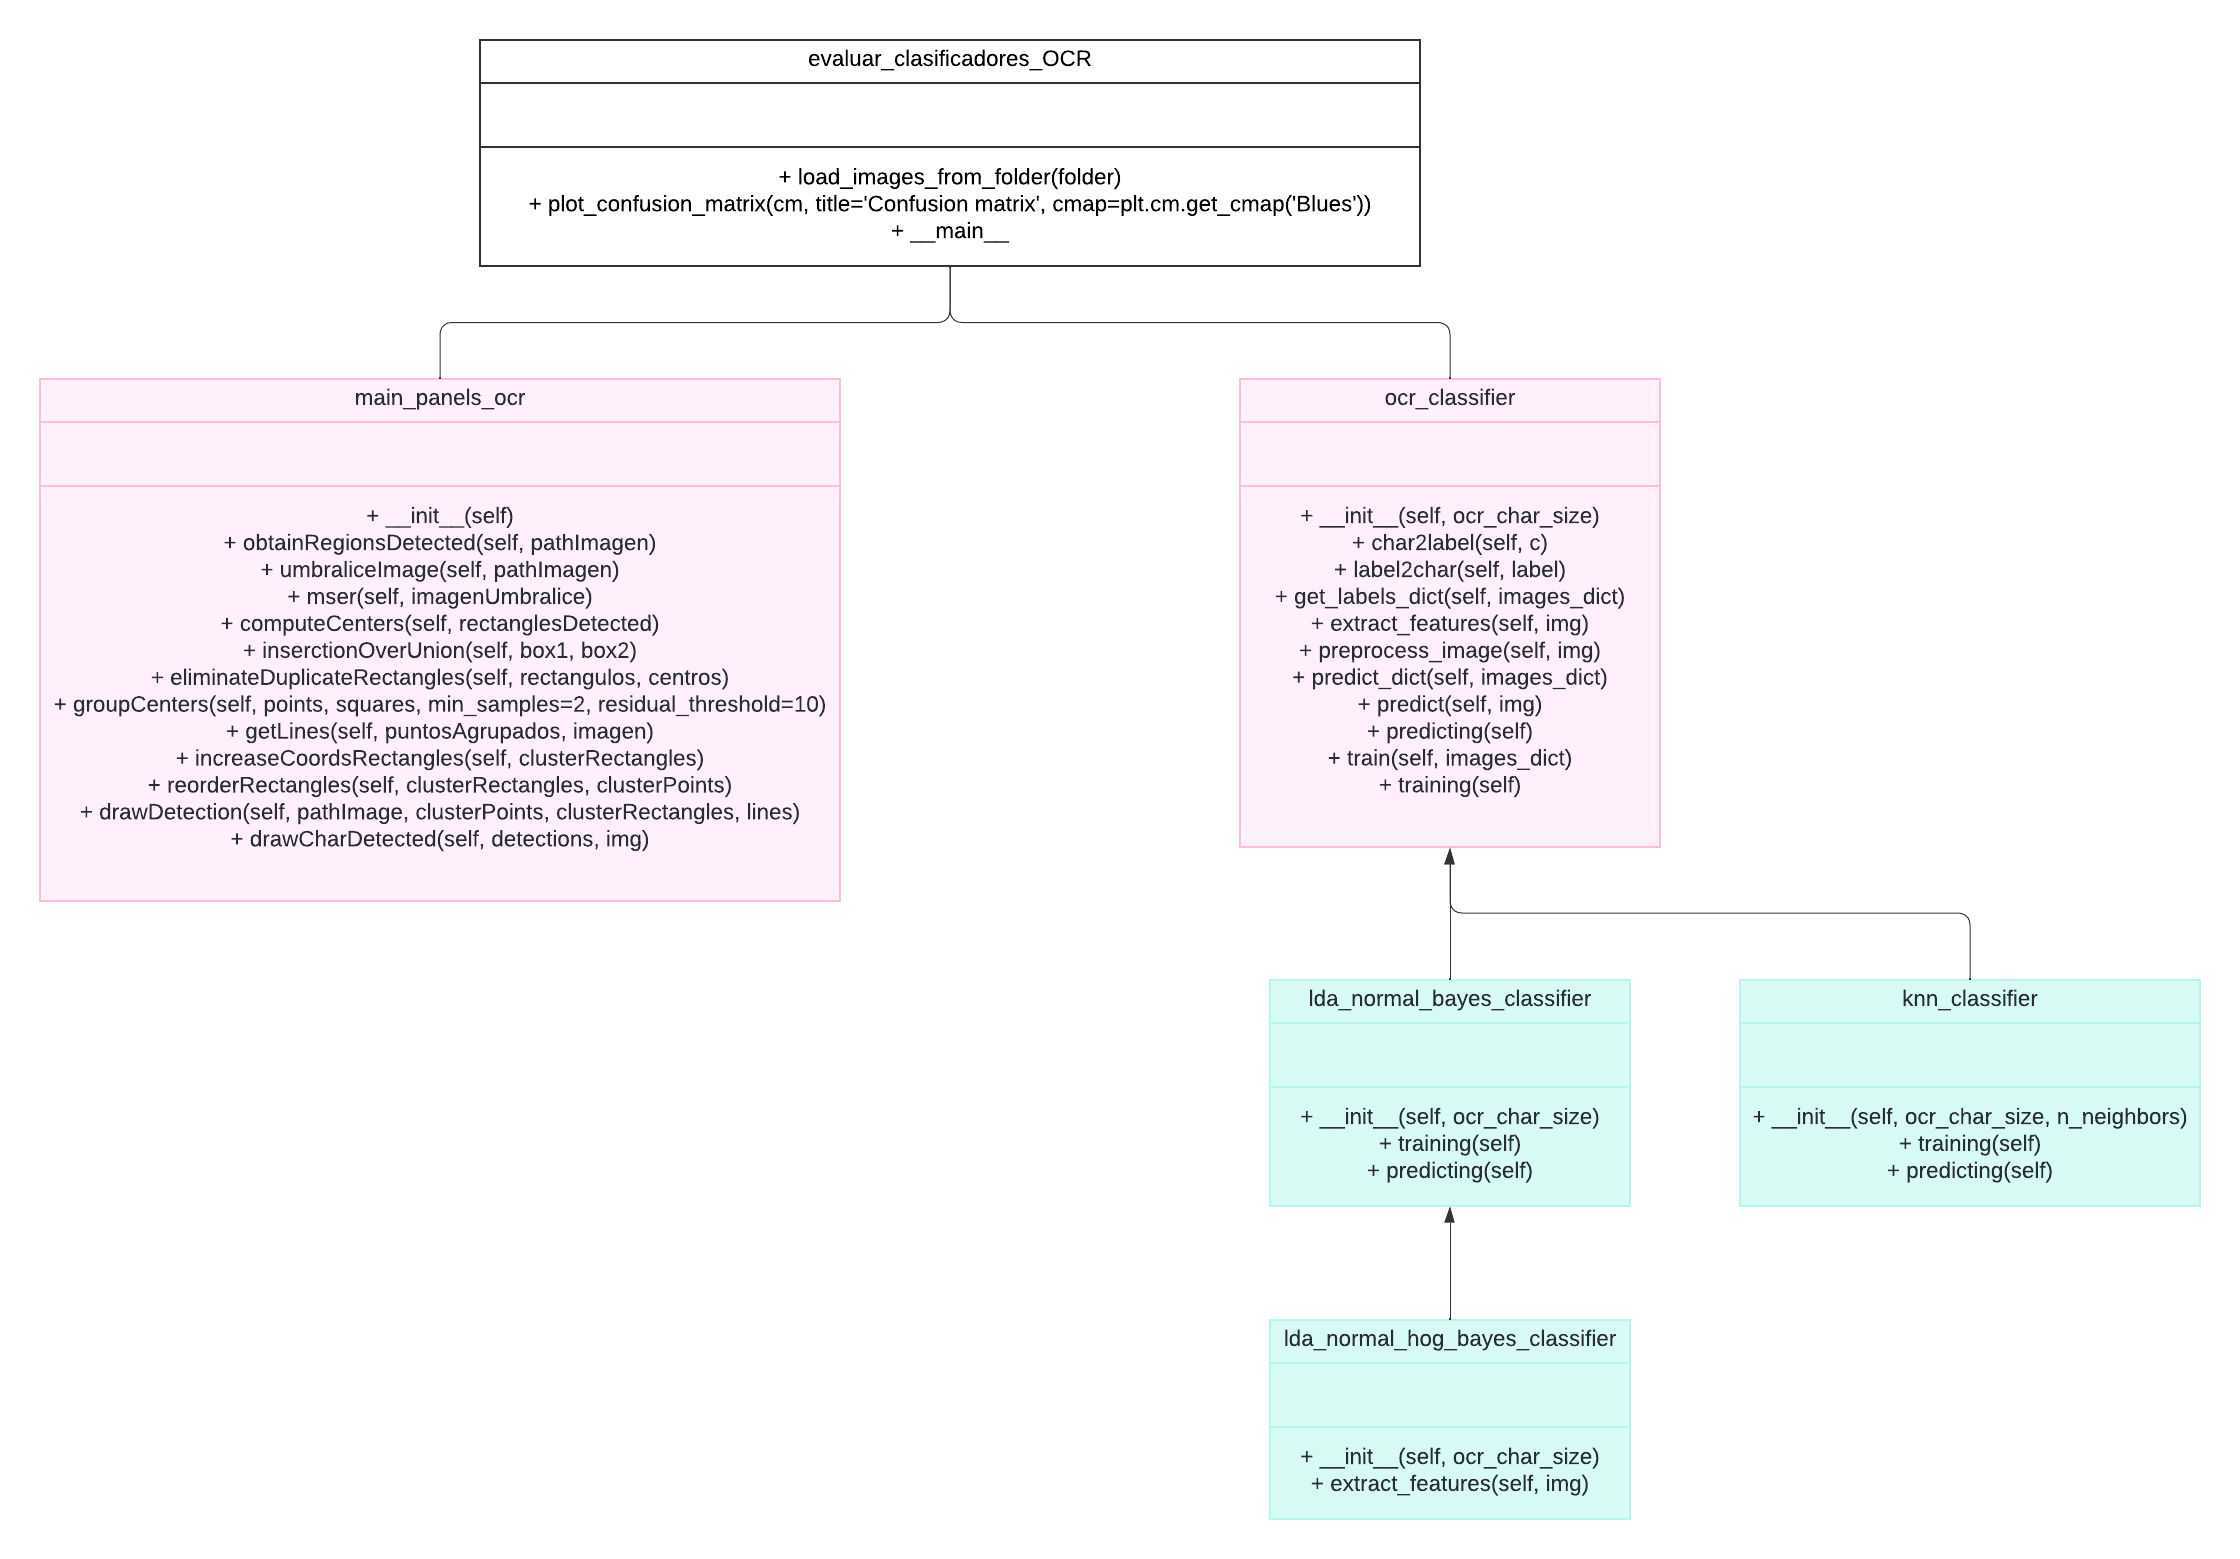
\includegraphics[width=1\linewidth]{./img/UML.png}
	\caption{Diagrama de clases}
	\label{fig:uml}
\end{figure}

En la \textbf{\hyperref[fig:uml] Fig. 1} vemos como estructura general del proyecto tenemos una clase \textit{main\_panels\_ocr} que se encarga de las fases de entrenamiento, validación y test, con carácteres extraidos de paneles, todo esto con ayuda de \textit{evaluar\_clasificadores\_OCR}.

Respecto a las clases relacionadas con los clasificadores tenemos a \textit{ocr\_classifier}, encargado de los métodos generales para todas las clases. A partir de aquí, \textit{lda\_normal\_bayes\_classifier} está como nuestro clasificador base y \textit{knn\_classifier} como primera alternativa a nivel de clasificador. 

Respecto a la segunda alternativa, hemos decidido partir de el clasificador base, y simplemente hemos decido cambiar el método de extracción de características, haciendo uso de HOG. Nótese que como solo cambia el método de extracción heredamos de \textit{ida\_normal\_bayes\_classifier}  y sobrescribimos el método.


\subsection{Ejercicio 1}
\textbf{Entrenamiento y validación de clasificadores de caracteres.}

Lo primero que se pide en este ejercicio es cargar y umbralizar las imágenes de los caracteres de entrenamiento, para ello hemos creado la función \textit{load\_images\_from\_folder} dentro del fichero \textit{evaluar\_clasificadores\_OCR}. El objetivo de esta función es cargar las imagenes del directorio que recibe como argumento. Se recorrerán las imágenes del directorio \textit{train\_ocr}, que es el directorio que pasamos en primer lugar, y cogerá el nombre de cada subdirectorio para crear una clave del mapa donde guardará las imagenes. Dentro del mapa, el valor asociado a cada clave será una lista de imágenes con las imágenes de los caracteres de esa clase, por ejemplo, para la clase 0 se guargará el 0 como clave del mapa y las imágenes del directorio con nombre 0, so guardarán como valor asociado a esa clave. 

En el caso de las letras es distinto porque tienes una estructura de ficheros distinta. Tenemos los ficheros \textit{Mayusculas} y \textit{minusculas} y dentro de estos ficheros tenemos los subdirectorios con las imágenes de cada letra. Por esto mismo cuando iteramos sobre los ficheros de \textit{train\_ocr} comprobamos si la \textit{label}, o nombre del directorio, es un digito porque en caso de serlo solo tenemos que usar el nombre como clave y las imágenes como valor, pero en caso de no ser un digito tenemos que iterar sobre sus subdirectorios donde ya si que podremos hacer el mismo proceso que hemos hecho con los números. 

La carga de las imágenes también será dentro del fichero \textit{evaluar\_clasificadores\_OCR} pero en el metodo \textit{main}. Después de hacer la carga de las imágenes de \textit{train\_ocr} también hacemos la carga de las imágenes de \textit{validation\_ocr} usando la misma función que con las anteriores.  

Para el umbralizado de las imágenes tenemos la función \textit{preprocess\_image}, dentro del fichero \textit{ocr\_clasifier} la utilizaremos para todas las imágenes, entrenamiento, validación y con las de test, ya que es importante que sea lo más parecido posible para todas las imagenes. En el caso de las imágenes de test tendremos que hacer alguna operación extra para que se parezcan lo más posible a las imagenes de entrenamiento como pasarlas a grises, ampliar la imagen añadiendole pixeles en los bordes o invertirlas, el resto de operaciones si que son las mismas. Esta función se va a llamar dentro de la función \textit{train} que está dentro del mismo fichero que la anterior. 

Para extraer las caracteristicas tenemos la función \textit{extract\_features}, a esta fucnión tambien la llamaremos desde \textit{train} y también se encuentra en el mismo fichero que las anteriores. Para el clasificador base esta función solo aplanará la imagen usando la función \textit{flatten}. Veremos en el ejercicio 2 que esta función cambiará para la creación de una de las variaciones del clasificador.

Dentro del metodo \textit{train} para cada una de las imagenes iremos ejecutando las dos funciones anteriores y además guardaremos el vector de caracteristicas de cada imagen en una matriz llamada \textit{C} y la clase a la que psertenece cada imagen en un vector de enteros lamado \textit{E}, para guardar el entero de las clases de letras guardaremos el valor de la tabla ascii. Una vez hemos hecho esto, convertimos la matriz y el vector en \textit{np.array} y usaremos la función \textit{fit\_transform} para encontrar la matriz de proyección y proyectar la matriz \textit{C} y convertirla en \textit{CR} y entrenaremos al clasificador con esta información. 

Para la validación tenemos que vover al fichero \textit{evaluar\_clasificadores\_OCR}. Una vez hemos terminado el entrenamiento vamos a validar los resultados de este. Usando las imagenes de \textit{validation\_ocr} vamos a ver en que clases clasificas las imágenes y comprobar si acierta con la clase a la que pertenecen originalmente. Para esto vamos a usar el método \textit{predict}, en este método preprocesa la imagen, extrae las características y reduce el vector de características, y con este vector reducido clasificamos la imagen correspondiente a este vector. Después de hacer esto se nos mostrará el valor de \textit{accuracy} indicando el porcentaje de acierto, que para el clasificador base será de 0.7130, este es tras hacer algunos cambios en el preprocesado de las imágenes ya que originalmente era de 0.952 pero no reconocía bien los caracteres que le pasabamos de los carteles, haciendo este cambio mejoró a la hora de reconocer los caracteres de los carteles pero empeoró el valor de \textit{accuracy}. Tambián mostrará la matriz de confusión donde podremos ver que clases son las que confunde a la hora de clasificar. 
Lo podemos ver en la \textbf{\hyperref[fig:normalizacion]{Fig. 2}}

\begin{figure}[h]
	\centering
	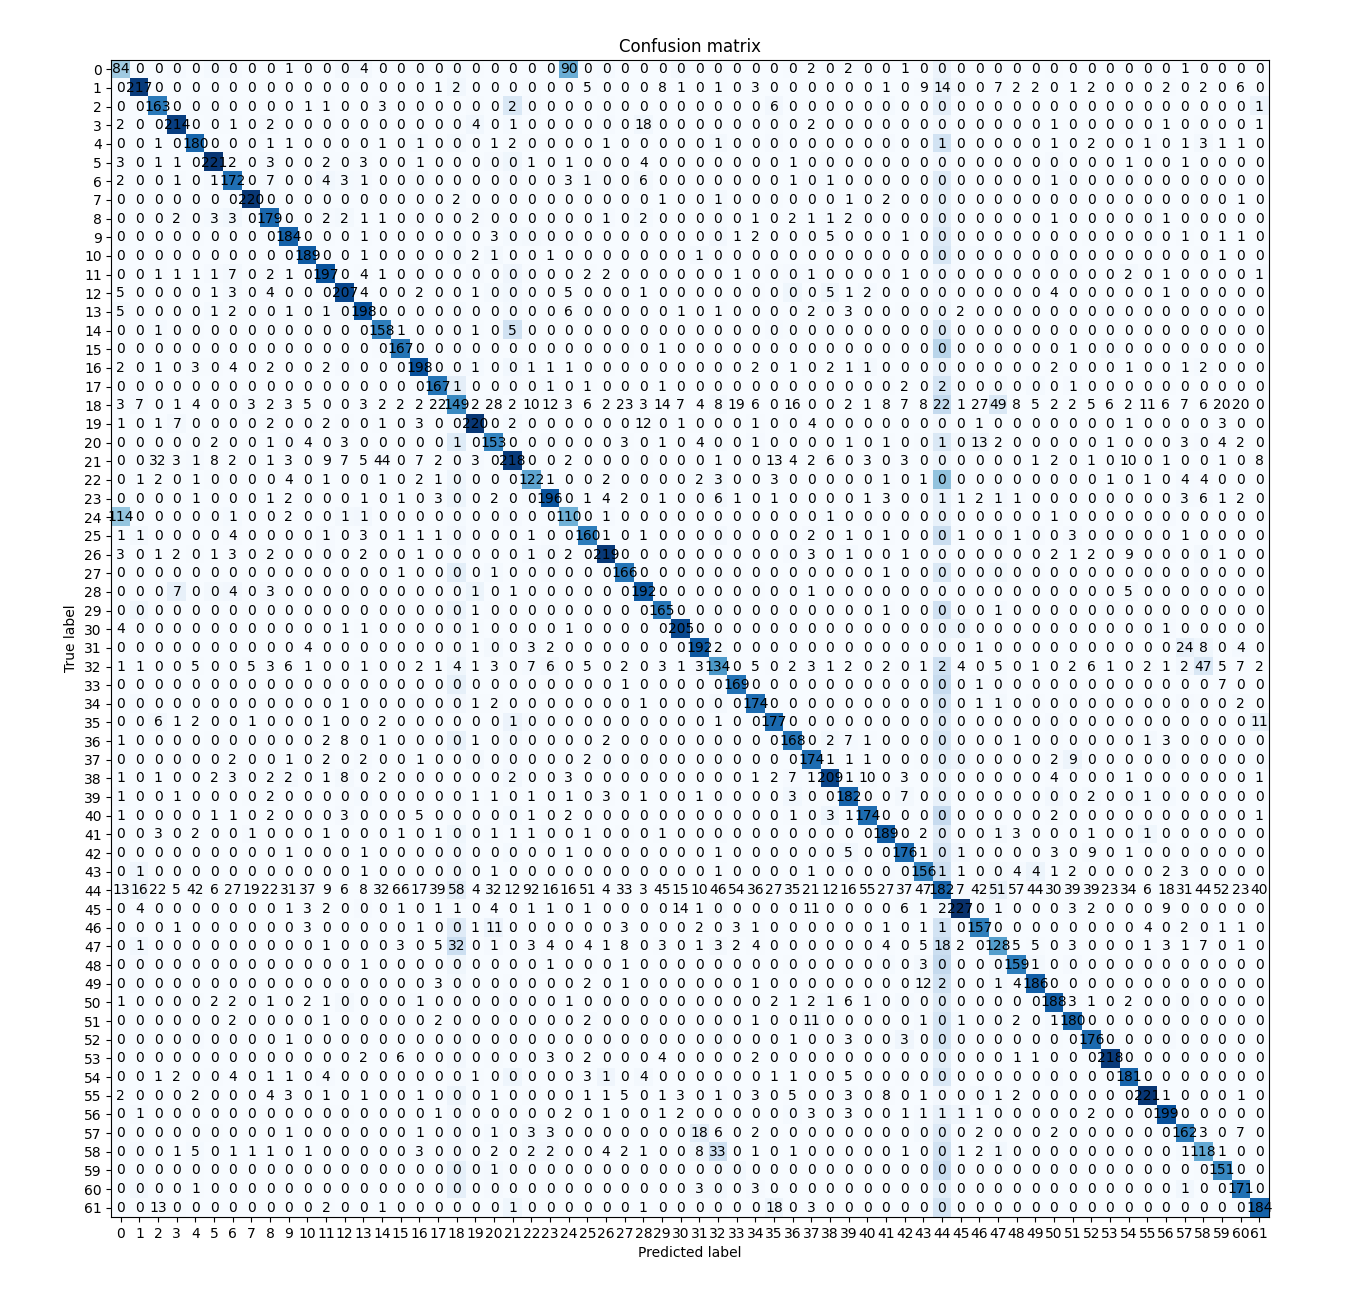
\includegraphics[width=0.9\linewidth]{img/matrixBase.png}
 	\caption{Matriz de confusión del clasificador base}\vspace{0.5cm}
	\label{fig:normalizacion}
\end{figure}


\subsection{Ejercicio 2}

\subsection{LDA, extraer vectores de características usando HOG}
Para crear una variante del clasificador base vamos a calcular el vector de características de una forma distinta a cuando lo calculamos para el clasificador base. 

El método \textit{extract\_features} tiene como objetivo extraer características HOG de una imagen proporcionada. HOG es una técnica para la extracción de características que es útil, especialmente, en tareas como el reconocimiento de objetos y la detección de movimiento.

La función para extraer las características la podemos encontrar en el fichero \\\textit{lda\_normal\_hog\_bayes\_classifier}. Dentro de esta función vamos a definir los parametros para el descriptor de HOG, el tamaño de la ventana de detección que será 25x25 píxeles, el tamaño de la agrupación de celdas o bloque que será 10x10 píxeles, el desplazamiento del bloque o cuántos píxeles se desplaza la ventana para calcular el siguiente bloque, el tamaño de la celda (celda es la unidad más pequeña de la que se calculan los histogramas de gradientes) y finalmente el número de contenedores para el histograma de gradiente. 

Después de definir estos parámetros creamos el descriptor y con el método \textit{compute} y usando la imagen como entrada podemos calcular las características, el resultado será una matriz que contiene los despcriptores HOG de la imagen. Finalmente con el método \textit{flatten} aplanamos la matriz y convertimos el array multidimensional en un vector unidimensional. 

El resto del proceso es igual que en las imagenges anteriores. 

Tras la ejecución del entrenamiento y la validación, el resultado de la \textit{accuracy} para este clasificador es de 0.728 mejorando los resultados del clasificador base. Como hemos dicho antes al hacer los cambios en el preproceado hemos conseguido mejorar la clasificación de los caracteres de los carteles pero ha empeorado el valor de validación, previamente para este clasificador era de más de 0.96. Podemos ver la matriz de confusión perteneciente a este clasificador en la  \textbf{\hyperref[fig:normalizacion]{Fig. 2}}

\begin{figure}[h]
	\centering
	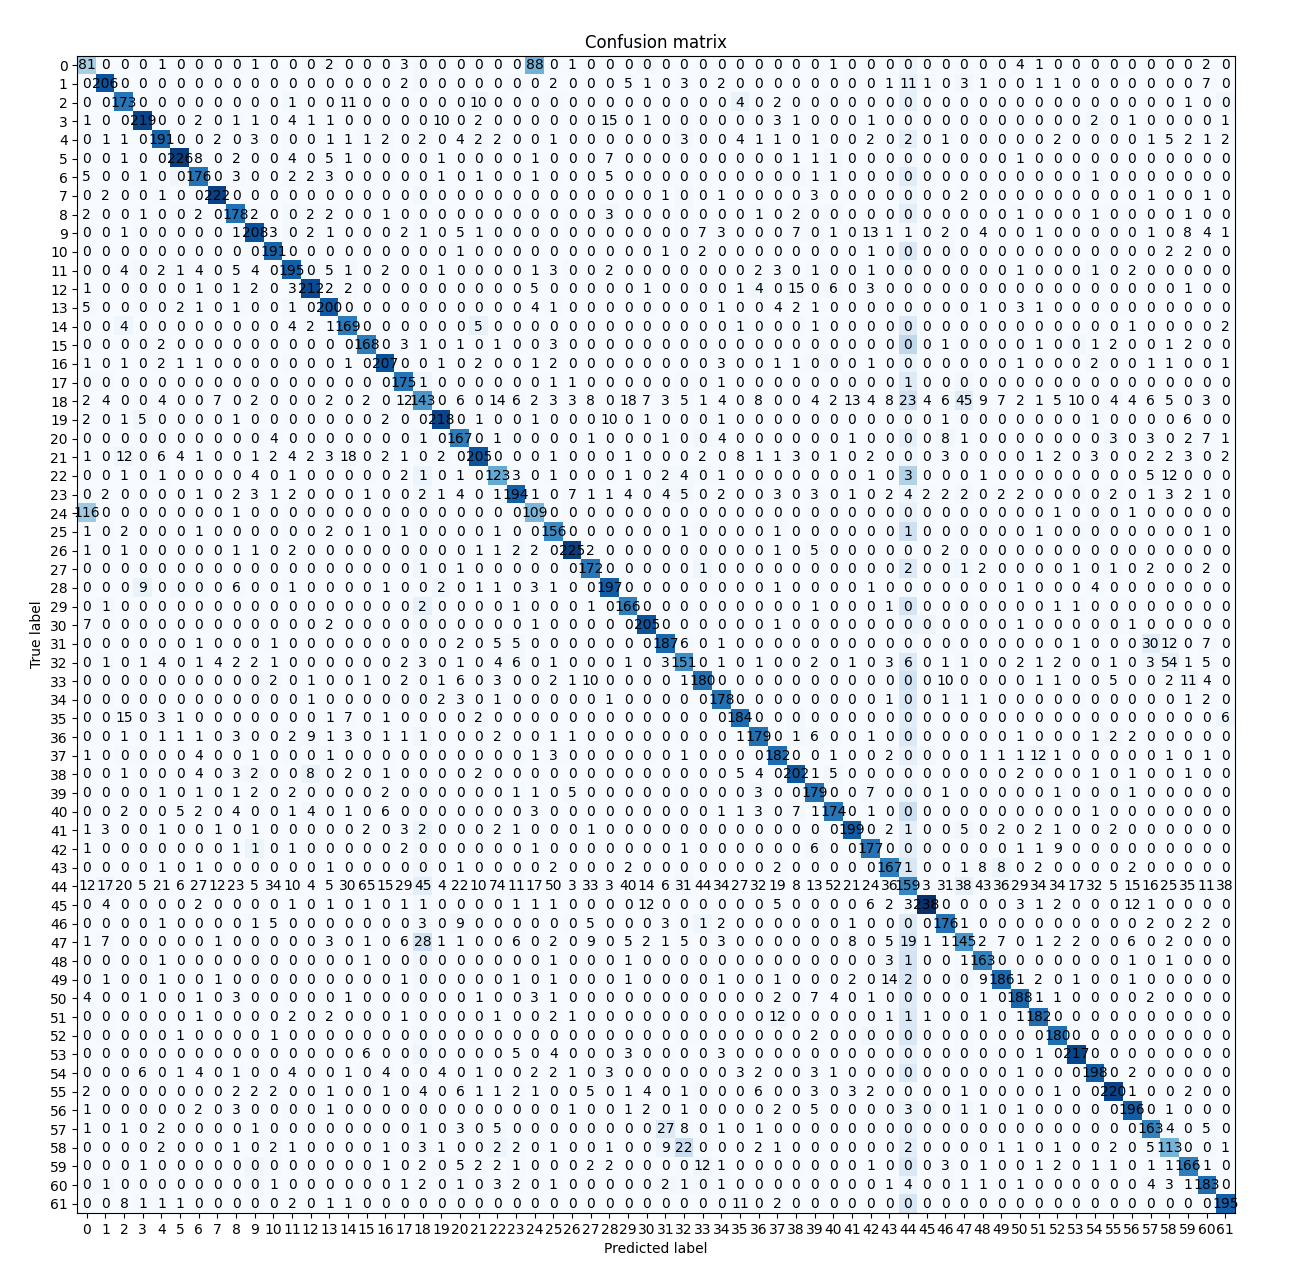
\includegraphics[width=0.9\linewidth]{img/matrixHOG.png}
 	\caption{Matriz de confusión del clasificador usando HOG}\vspace{0.5cm}
	\label{fig:normalizacion}
\end{figure}


\subsubsection{KNN}
El algoritmo \textbf{K-Nearest Neighbors (KNN)} es un método de clasificación supervisada que asigna una clase a una entrada fijándonos en las clases de sus $k$ vecinos más cercanos en un espacio de características. 

El funcionamiento básico del KNN es el siguiente:

\begin{quote}
	\textbf{1. Selección de Vecinos:} Dado un valor de k, el algoritmo selecciona los k vecinos más cercanos a la muestra que se desea clasificar. La cercanía se mide típicamente utilizando una distancia, como la distancia Euclidiana.
	
	\textbf{2. Asignación de Clase:} La clase de la muestra se determina por mayoría de votos entre los k vecinos seleccionados. La clase más frecuente entre estos vecinos se asigna a la muestra. Si hay un empate, se puede decidir la clase de la muestra de diferentes maneras, como elegir la clase del vecino más cercano.
	
	\textbf{3. No Paramétrico:} El KNN es un clasificador no paramétrico, lo que significa que no hace suposiciones sobre la distribución de los datos.
	
\end{quote}

\textbf{Consideraciones para la Implementación}

\begin{quote}
	\textbf{Elección del valor de $k$:}
	\begin{quote}
		\textbf{Influencia de k:} El valor de k tiene una gran influencia en el rendimiento del clasificador. Un k muy pequeño puede hacer que el modelo sea sensible al ruido en los datos, mientras que un k muy grande puede hacer que el modelo sea demasiado general y no capture bien las peculiaridades de las diferentes clases.
	\end{quote}
	
	\begin{quote}
		\textbf{Selección de k:} En general, k se elige utilizando técnicas de validación cruzada. Se prueban diferentes valores de k y se selecciona el que ofrece el mejor rendimiento.
	\end{quote}
	
\end{quote}

\textbf{Resultados}

El clasificador KNN con 3 vecinos alcanzó una precisión del 71.3\%, superando el 72.65\% obtenido con el clasificador base. A continuación, se presenta una comparación de los resultados:

\begin{quote}
	- Precisión del Clasificador Base: 0.713\%
	
	- Precisión del Clasificador KNN: 0.7265\%
\end{quote}

Además, en la \textbf{\hyperref[fig:matrixknn] Fig. 4} se generó una matriz de confusión que muestra la distribución de errores y aciertos del clasificador KNN. Esta matriz ayuda a identificar las clases que se confunden con mayor frecuencia, proporcionando información valiosa para futuras mejoras.

\textbf{Razones de mejora}

El clasificador \textbf{KNN} puede ofrecer mejores resultados en este contexto por varias razones:
\begin{quote}
	\textbf{1. Robustez ante Variabilidad y Ruido:} Dado que KNN toma en cuenta múltiples vecinos, es menos sensible a pequeñas variaciones y ruido en los datos. Esto es especialmente útil en el reconocimiento de caracteres donde puede haber distorsiones y ruido en las imágenes.

	\textbf{2. Simplicidad y Eficacia:} KNN es simple de implementar y puede ser muy efectivo cuando se dispone de una cantidad adecuada de datos de entrenamiento. 
	
\end{quote}

Además hay que resaltar que \textbf{KNN} tiene una gran adaptabilidad, por lo que puede adaptarse fácilmente a nuevas clases de caracteres sin necesidad de un retraining. Solo se necesita agregar nuevas muestras al conjunto de datos.

\begin{figure}[h]
	\centering
	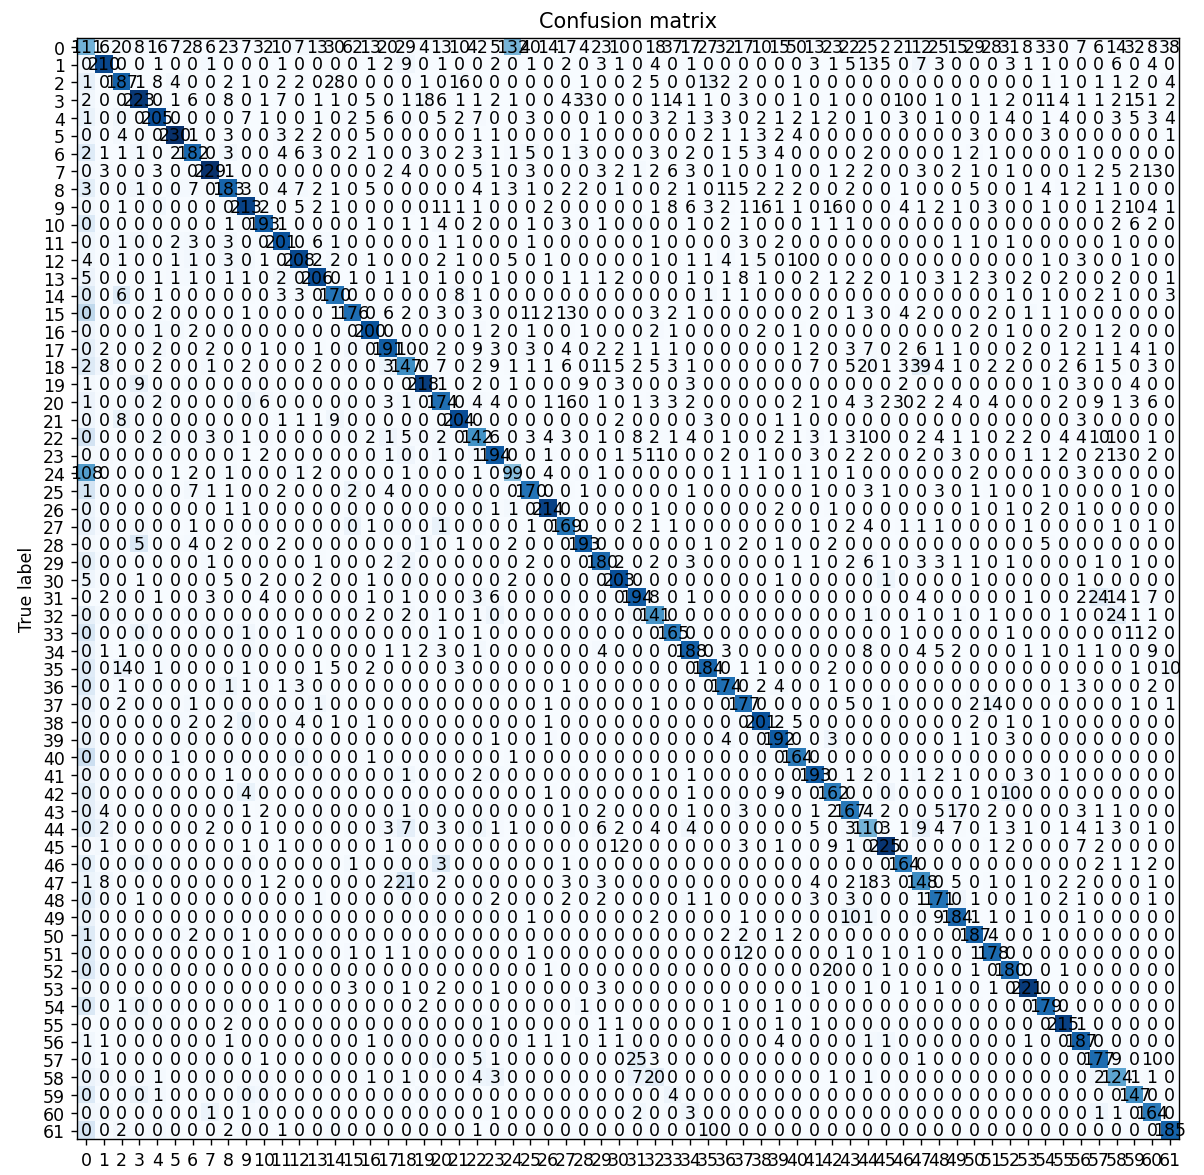
\includegraphics[width=0.7\linewidth]{img/matrixKNN.png}
	\caption{Matriz de confusión del clasificador KNN}
	\label{fig:matrixknn}
\end{figure}

\subsection{Ejercicio 3}
Una vez hemos conseguido entrenar un clasificador de caracteres y quedarnos con el que mejor resultados da, vamos a aplicar ese modelo a un caso más real que sería a la hora de detectar carteles de una autopista y clasificar los caracteres que se encuentran en el panel. La clase encargada de realizar toda esta parte de la lectura automática de los caracteres es \textit{main\_panels\_ocr.py}, donde llamando al método \textit{obtainRegionsDetected} podemos obtener los parámetros necesarios para la realización de este apartado. \\\\
Las imágenes con las que queremos realizar esta lectura son de unos carteles recortados de forma, orientación y relación de aspecto variable. Nuestro primer paso consiste en poder detectar los caracteres que luego vamos a clasificar. Para ello previamente vamos a normalizar el panel que le entre a este detector, donde primero cargaremos la imagen en escala de grises, aplicaremos un umbralizado adaptativo aplicando la Gaussiana y por último extraemos los bordes de la imagen umbralizada. El proceso que se ha seguido se puede ver a partir de la \textbf{\hyperref[fig:normalizacion]{Fig. 5}}
\newpage
\begin{figure}[h]
	\centering
	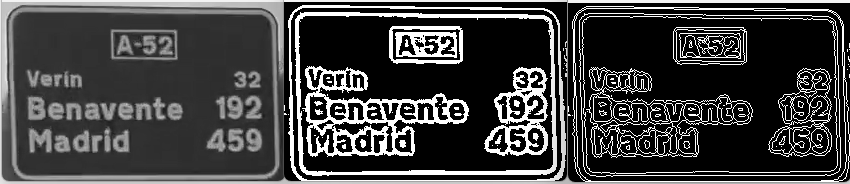
\includegraphics[width=0.8\linewidth]{img/imagenUmbral.png}
 	\caption{Proceso de normalización para la lectura de carteles}\vspace{0.5cm}
	\label{fig:normalizacion}
\end{figure}
Después de la umbralización, vamos a usar MSER para poder detectar las regiones más características de nuestra imagen, en este caso caracteres. La imagen se le pasará al método y antes de realizar el MSER realizaremos una dilatación para aumentar el grosor de los trazos de los caracteres. Los parámetros del MSER escogidos son los siguientes:
\begin{itemize}
    \item Delta = 5
    \item Variación máxima = 0.8
    \item Área mínima = 50
    \item Área máxima = 200
\end{itemize}
Lo más destacable de estos parámetros es la disminución de la ventana de las regiones detectadas debido a que nos encontramos con imágenes con bastante menos píxeles que las imágenes de la práctica anterior, donde nos encontrábamos con una imagen de toda la escena. El método devolverá una lista compuesta por las coordenadas de cada rectángulo detectado. En la \textbf{\hyperref[fig:normalizacion]{Fig. 6}} vemos cómo se comporta esta detección. 
\begin{figure}[h]
	\centering
	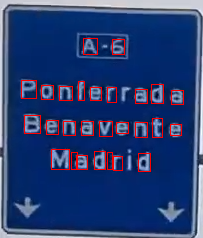
\includegraphics[width=0.2\linewidth]{img/deteccionMSER.png}
 	\caption{Carteles detectados con MSER}\vspace{0.5cm}
	\label{fig:normalizacion}
\end{figure}
\\Puede suceder que MSER detecte varias regiones que pertenecen a un mismo carácter. Esto se soluciona cuando se llama al método \textit{eliminateDuplicatedRectangles}, donde itera todos los rectángulos detectados y comprueba si dos de los rectángulos iterados se encuentran contenidos. Para saber eso se calcula un valor de IoU, donde a partir de un umbral podemos saber si dos rectángulos están superpuestos. Cuando nos encontremos en este caso, eliminaremos el rectángulo que abarque menos área y nos quedaremos con el más grande de los dos. Este bucle se recorrerá para todos los detectados.
\\\\
El paso siguiente consiste es poder agrupar los caracteres en palabras. Por ejemplo en el anterior cartel de la \textbf{\hyperref[fig:normalizacion]{Fig. 6}} a partir de los caracteres detectadas queremos formar el texto \textit{A6 Ponferrada Benavente Madrid}. La clase llama primero a la función \textit{computeCenters} que devolverá una lista con las coordenadas de los centros de los rectángulos. Esto se hace para poder ejecutar el algoritmo de RANSAC que se encargará de realizar esta agrupación. El método en cuestión es \textit{gropuCenters} y los parámetros serán los puntos y rectángulos a procesar y el número mínimo de muestras que compone una línea, donde en nuestro caso queremos formar palabras de más de 1 carácter, y un umbral de residuo que se utiliza para ajustar las líneas y diferenciar si una línea pertenece o no a un punto en función de su valor, que sería la distancia entre dos puntos. El algoritmo de RANSAC se aplicará a cada uno de los puntos. Para una mejor visión del algoritmo, nos centraremos en el ejemplo de la \textbf{\hyperref[fig:normalizacion]{Fig. 7}}.
\begin{figure}[h]
	\centering
	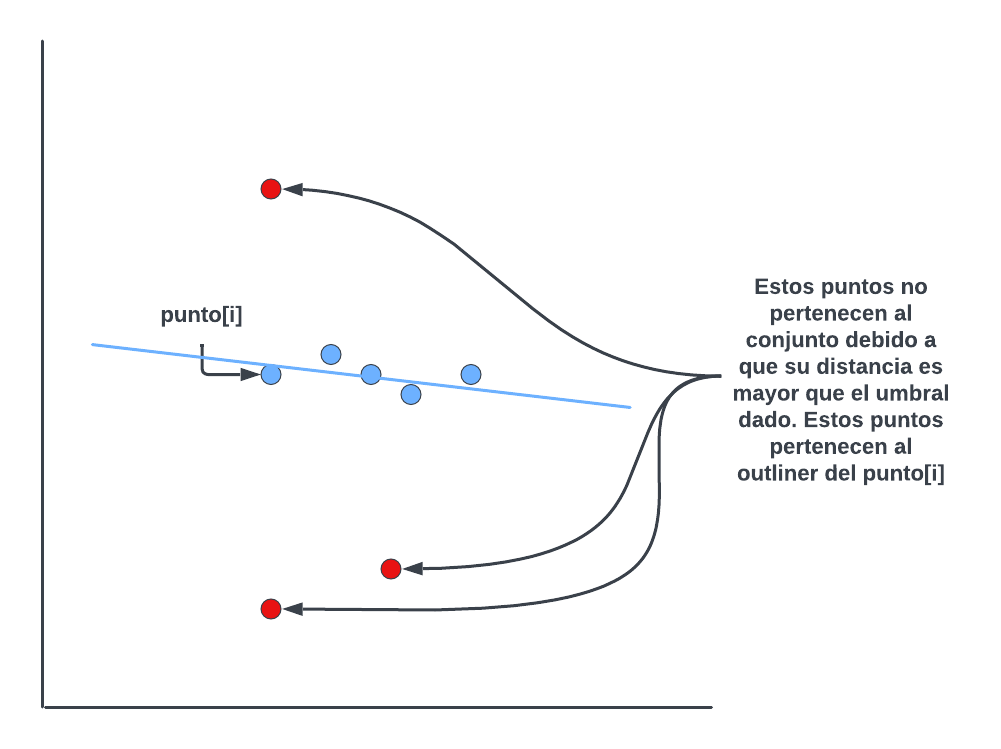
\includegraphics[width=0.6\linewidth]{img/RANSAC.png}
 	\caption{RANSAC aplicado a los puntos detectados}\
	\label{fig:normalizacion}
\end{figure}
\\ En la figura vemos que nos encontramos con el punto i de nuestro bucle. Sobre ese punto intentaremos obtener la línea de RANSAC a partir del umbral de residuo. Si un punto se encuentra a una mayor distancia que el umbral entonces el algoritmo no lo tendrá en cuenta a la hora de trazar la recta. Vemos que los puntos de arriba y abajo no deberían de pertenecer a la palabra ya que se encuentran más alejados que los que están en los puntos de en medio. La función de RANSAC tiene del método \textit{inlier\_mask} que permite calcular los puntos que pertenecen a la recta calculada. El método en cuestión devolverá una mascará que tendrá la misma longitud que la lista de los puntos y nos dirá  los puntos que se encuentran en el subconjunto. Esos puntos los almacenaremos en una lista de conjuntos y los marcaremos como explorados, para evitar que uno de los puntos obtenidos de la recta se itere otra vez. En el ejemplo la siguiente iteración será uno de los puntos de abajo o el de arriba ya que los puntos de en medio ya han sido explorados y se realizará el mismo proceso que lo anterior explicado. En este caso tendremos dos subconjuntos: los puntos de en medio y los puntos de abajo. El punto de arriba no ha sido agregado a ningún punto ya que los mínimos de puntos que hemos establecido para establecer la línea de RANSAC son dos. El proceso que se acaba de explicar, se puede ver a través de la siguiente figura \textbf{\hyperref[fig:puntosAgrupados]{Fig. 8}}.
\begin{figure}[h]
	\centering
	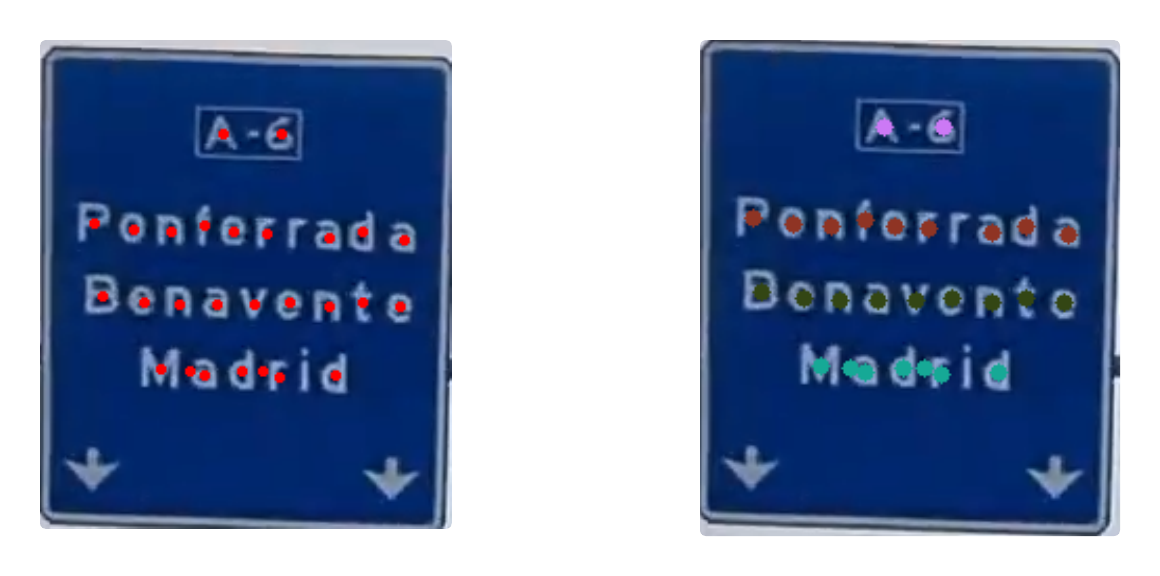
\includegraphics[width=0.6\linewidth]{img/puntosAgrupados.png}
 	\caption{Cálculo y agrupación de los centros de los rectángulos mediante RANSAC}\
	\label{fig:puntosAgrupados}
\end{figure}
\\El proceso de la detección de las palabras ya estaría completado, donde ya se han obtenido todas las líneas, rectángulos y centros detectados sobre la imagen, véase \textbf{\hyperref[fig:imagenDetectada]{Fig. 9}}. Nuestro último paso sería pasarle una lista de conjuntos de caracteres al clasificador para poder saber el tipo de carácter y así poder construir el texto del panel. Sin embargo, los paneles están desordenados, por lo que se construirá un texto erróneo ya que las palabras no están en orden. Para ello antes de realizar la clasificación se llama al método \textit{reorderRectangles}. El algoritmo es muy sencillo aunque es un tanto extenso. Las palabras deberían estar ordenadas en como leemos nosotros el texto, de arriba a abajo, y los caracteres de izquierda a derecha. Primero reordenaremos las palabras para que estén de arriba a abajo. Para ello, nuestra variable \textit{clusterRectangles} es una lista 
\begin{figure}[h]
	\centering
	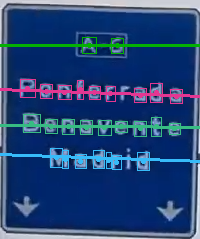
\includegraphics[width=0.2\linewidth]{img/detectionPanel.png}
 	\caption{Detección caracteres panel}\
	\label{fig:imagenDetectada}
\end{figure}
\\de listas, donde cada posición es la oración en sí. Iteraremos cada una de las oraciones y calcularemos su posición respecto al eje Y y reordenaremos esta lista de manera ascendente, donde las oraciones con menor Y irán primeras y las oraciones con mayor Y las últimas. Cabe destacar que en imágenes el punto (0,0) corresponde a la parte superior izquierda y es por esto por lo que se reordena en función del Y menor. Una vez hemos realizado el primer reordenamiento, podemos hacer el reordenamiento a nivel de carácter. Para ello en vez de usar los conjuntos de las listas, usaremos los conjuntos de los conjuntos de las listas, que representan a cada palabra de una oración. Sobre cada palabra aplicaremos un reordenamiento muy similar al anterior pero en este caso usando el eje X en lugar del Y. 
\\\\ Por último, después de realizar con éxito toda la detección de los caracteres, su composición en palabras y en oraciones separadas por saltos de línea, el siguiente y último paso será la calorificación de los caracteres y la construcción del texto. Se iterará cada conjunto de palabras y se volverá a iterar para obtener el carácter. El carácter se le pasará al clasificador que hayamos seleccionado: Normal Bayesiano, Normal Bayes con Hough y el KNN. Pese a que obtuvimos una gran precisión durante el entrenamiento y validación de los tres modelos, los tres superaban el 90\% precisión, la mayoría de los caracteres los clasifica de forma errónea. Uno de los problemas que tuvimos en un principio era que el carácter recortado obtenido por MSER estaba demasiado cerca, a diferencia del conjunto de entrenamiento donde los caracteres estaban centrados, eran más finos y estaban más alejados. Para solucionar esto, antes de clasificar normalizamos el carácter para mejorar los resultados como se puede ver en la \textbf{\hyperref[fig:imagenDetectada]{Fig. 10}}.
\newpage
\begin{figure}[h]
	\centering
	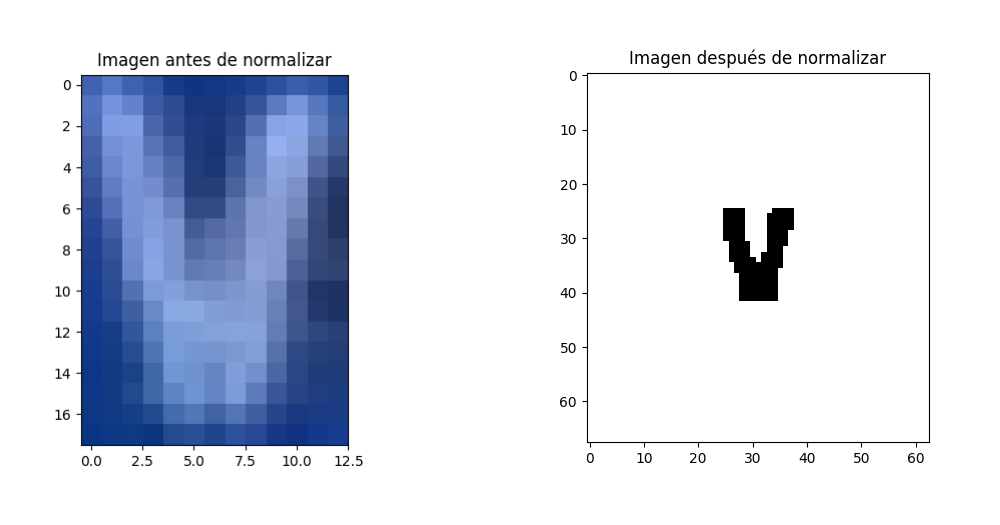
\includegraphics[width=0.6\linewidth]{img/imgNorm.png}
 	\caption{Detección caracteres panel}\
	\label{fig:imagenDetectada}
\end{figure}
La normalización consiste en pasarla a una escala de grises, añadirle un padding para que el carácter se muestre más alejado, se invierte la imagen, se le aplica un suavizado Gaussiano, se umbraliza la imagen para tener una imagen con dos valores de píxeles y finalmente se le aplica una apertura para reducir el ruido. Después de esta normalización se redimensiona la imagen a una escala de 25x25 para que tengan el mismo formato que las imágenes de entrenamiento. Aunque ahora los caracteres que le pasamos al clasificador son muy similares a como fue entrenado el modelo, sigue dando resultados erróneos, como se puede ver en la \textbf{\hyperref[fig:imagenClasificada]{Fig. 11}}.

\begin{figure}[h]
	\centering
	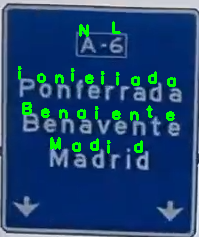
\includegraphics[width=0.3\linewidth]{img/imagenClasificada.png}
 	\caption{Cartel clasificado}\
	\label{fig:imagenClasificada}
\end{figure}

Podemos probar de otra forma la eficiencia de nuestro algoritmo y es mediante el uso de la clase \textit{evaluar\_resultados\_test\_ocr\_panels.py} que se proporciona en el enunciado. Esta clase si se ejecuta realiza una comparación entre el fichero de ground truth, que tiene el texto real, y el fichero que hemos generado nosotros, donde contiene las palabras construidas por el algoritmo. La gráfica generada que se muestra en la \textbf{\hyperref[fig:levenshtein]{Fig. 12}} representa la distancia de Levenshtein, que sería el número mínimo de operaciones que se tiene que realizar para transformar una cadena en otra. 
\begin{figure}[h]
	\centering
	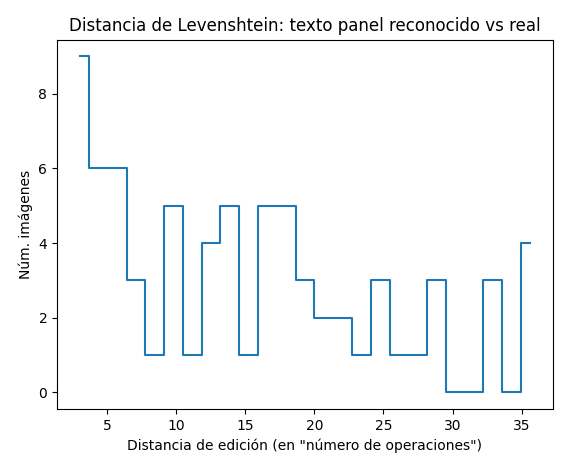
\includegraphics[width=0.5\linewidth]{img/Levenshtein.png}
	\caption{Distancia de Levenshtein}\
	\label{fig:levenshtein}
\end{figure}
\\Vemos que hay algunos paneles que se encuentran por debajo de 2 e incluso alguno con 0. Sin embargo, pese a tener unas distancias bastante buenas, el texto generado se asemeja muy poco con el texto real. Cabe destacar que para generar las salidas del texto se ha usado el detector Bayesiano normal con Hogh que tiene una precisión del 0.72.

\section{Conclusión}
En esta práctica, desarrollamos un sistema OCR para leer paneles informativos en autopistas. Probamos varios clasificadores, destacando la versión con HOG, que alcanzó una precisión del 72.8\% en el conjunto de entrenamiento. Sin embargo, al aplicar el sistema a paneles reales, los resultados fueron menos precisos debido a la variabilidad de los caracteres y las condiciones del entorno.

A pesar de un preprocesamiento exhaustivo, los errores en la clasificación indicaron la necesidad de seguir mejorando los métodos utilizados. En general, aunque se lograron avances significativos, es necesario continuar refinando el sistema para obtener una mayor precisión en aplicaciones prácticas.
\end{document}
